% pdflatex relatorio_porosidade_ml.tex (executar neste diretorio)

\documentclass[12pt,a4paper]{article}

\usepackage[T1]{fontenc}
\usepackage[utf8]{inputenc}
\usepackage[brazil]{babel}
\usepackage{microtype}
\usepackage{graphicx}
\usepackage{booktabs}
\usepackage{amsmath}
\usepackage{hyperref}
\usepackage{geometry}
\usepackage{tikz}
\usetikzlibrary{arrows.meta,positioning}
\geometry{margin=2.5cm}

\graphicspath{{figs/}}

\title{Regressão supervisionada de porosidade a partir de perfis convencionais:\\
diagnóstico de colinearidade e leitura crítica das métricas}
\author{}
\date{\today}

\begin{document}
\maketitle

\begin{abstract}
Trata-se do registro analítico de um ensaio de regressão para estimar porosidade
a partir de curvas de perfilagem: intervalo de trânsito sônico (AC), densidade
aparente \(\rho_b\), impedância acústica (AI), velocidade da onda de compressão
P (\(V_p\)), raio gama (GR) e variável associada à fração argilosa (\(V_c\)).
O ajuste emprega um modelo GBDT (\textit{Gradient Boosting Decision Trees}, conjunto
de árvores de decisão com reforço por gradiente, aqui na variante baseada em
histogramas). A avaliação usa partição treino--teste ao longo da profundidade;
por \textbf{teste profundo}, equivalente neste documento a \textbf{bloco de teste profundo},
entende-se o conjunto das \(20\%\) observações com maior profundidade após ordenar o
conjunto tabular pela profundidade mecânica registada ao longo da coluna, mantendo o treino na fração rasa
complementar. Descrevem-se ainda ablações de preditores e o diagnóstico multivariado: correlações de Pearson
e de Spearman e fator de inflação da variância (VIF) no treino; informação mútua
(MI) entre cada preditor e a porosidade também no treino; importância por permutação do
coeficiente de determinação (\(R^2\)) no teste, e valores SHAP
(\textit{SHapley Additive exPlanations}, decomposição aditiva do efeito de cada
preditor com base em Shapley). Complementam o quadro, no conjunto de teste profundo,
o erro absoluto médio (MAE, do inglês \textit{mean absolute error}) e a raiz do
erro quadrático médio (RMSE, \textit{root mean squared error}). No \textbf{recorte
principal}, sob partição treino--teste ao longo da profundidade e com as curvas
tal como apresentadas nas figuras deste relatório, \(V_p\) e a impedância acústica (AI) não acrescentam
\textbf{ganho preditivo marginal detectável} quando AC e \(\rho_b\) já entram no
modelo: o \(R^2\) no teste profundo permanece praticamente inalterado após retirá-los.
Isto documenta redundância preditiva \textbf{local} nesse protocolo, não
irrelevância física universal dessas grandezas. Os resultados devem ser lidos como
evidência de colinearidade e redundância no recorte analisado, \textbf{não} como
demonstração de generalização entre poços ou entre contextos geológicos
distintos.
\end{abstract}

\section{Introdução}\label{sec:intro}

A porosidade controla, com mineralogia e fluido, a resposta elástica efetiva da
rocha. Em colunas perfiladas, relações empíricas entre porosidade e
grandezas sônicas ou de densidade são esperadas; o mesmo vale para grandezas
derivadas da combinação massa--rigidez, como a impedância acústica (AI) e a
velocidade da onda de compressão P (\(V_p\)). Daí decorre um risco metodológico: modelos supervisionados
podem atingir erros baixos no teste sem que isso signifique, por si só, que cada
preditor contribua com informação independente.

Os achados de ablação não implicam irrelevância física de \(V_p\) ou de AI,
mas sim \textbf{ausência de contribuição preditiva marginal detectável} no
recorte considerado, dado o forte acoplamento dessas grandezas com AC e \(\rho_b\) e a
qualidade relativa das curvas usadas como entrada.

O objetivo deste texto é documentar, com rigor modesto porém explícito, um
baseline de regressão e o diagnóstico que o acompanha. Pretende-se responder,
com base em números e figuras, se a retirada isolada de \(V_p\) ou da impedância
acústica (AI) altera o desempenho, e se correlações e o fator de inflação
da variância (VIF) sustentam a
leitura de redundância entre preditores. Inclui-se ainda um contraste entre dois
recortes verticais distintos, para lembrar que a generalização entre contextos
não se infere apenas de \(R^2\) alto num único intervalo.

\section{Quadro teórico sucinto}\label{sec:fund}

Em meio efetivo, a impedância acústica \(Z\) relaciona massa volumétrica
\(\rho\) e velocidade \(V\) segundo
\begin{equation}\label{eq:impedancia}
Z = \rho\,V .
\end{equation}
Quando \(\rho\) e \(V\) são estimados a partir das mesmas observações que
alimentam o intervalo de trânsito, a informação trazida por \(Z\) tende a
sobrepor-se à de \(V\) e à de \(\rho\), em vez de acrescentar graus de liberdade
estatísticos novos.

Para avaliar o ajuste global no teste, utilizou-se o coeficiente de determinação
\begin{equation}\label{eq:r2}
R^2 = 1 - \frac{\sum_{i=1}^{n}(y_i - \hat{y}_i)^2}{\sum_{i=1}^{n}(y_i - \bar{y})^2},
\end{equation}
onde \(y_i\) é a porosidade observada, \(\hat{y}_i\) a predição e \(\bar{y}\)
a média amostral no conjunto de teste de cardinalidade \(n\). O erro absoluto
médio (MAE) foi
\begin{equation}\label{eq:mae}
\mathrm{MAE} = \frac{1}{n}\sum_{i=1}^{n} \lvert y_i - \hat{y}_i\rvert ,
\end{equation}
isto é, o erro absoluto médio (MAE, do inglês \textit{mean absolute error}). A
raiz do erro quadrático médio (RMSE, \textit{root mean squared error}) foi
\begin{equation}\label{eq:rmse}
\mathrm{RMSE} = \sqrt{\frac{1}{n}\sum_{i=1}^{n}(y_i - \hat{y}_i)^2}\,.
\end{equation}
Estas grandezas resumem o encaixe, mas não distinguem, por si só, contribuição
marginal de preditores correlacionados.

\section{Questões de trabalho}\label{sec:perguntas}

Colocam-se as seguintes questões, respondidas na Secção~\ref{sec:discussao}
com apoio nas Figuras~\ref{fig:f03vp}--\ref{fig:shap} e na Tabela~\ref{tab:metricas}:

\begin{enumerate}
  \item O erro de generalização no bloco de teste profundo muda de forma
  relevante quando se retira \(V_p\), quando se retira a impedância, ou ambas?
  \item As estruturas de correlação e o fator de inflação da variância
  (VIF, medida clássica de colinearidade em regressão linear auxiliar) indicam
  colinearidade forte o suficiente para explicar a estabilidade de \(R^2\) sob
  ablação?
  \item A importância por permutação do \(R^2\) e o resumo SHAP
  (\textit{SHapley Additive exPlanations}) apontam para um preditor dominante entre os
  elásticos?
  \item O mesmo protocolo, aplicado a um segundo recorte vertical, produz \(R^2\)
  sensivelmente diferente?
\end{enumerate}

\section{Metodologia}\label{sec:metodo}

\subsection{Dados e variáveis}
Utilizou-se um perfil tabular com sete preditores: intervalo de trânsito (AC),
densidade aparente \(\rho_b\), impedância acústica (AI), velocidade \(V_p\),
raio gama (GR), variável associada à argila (\(V_c\)) e porosidade como alvo.

Neste relatório, \textbf{recorte} designa um \textbf{trecho vertical} da coluna
perfilada analisado através de um \textbf{conjunto tabular 7logs completo}
(preditor + alvo), com amostragem regular ao longo da profundidade e
\textbf{identificador de amostra} próprio (etiqueta convencional do recorte vertical
considerado). O \textbf{recorte principal} corresponde à etiqueta F03-4; o
\textbf{recorte de contraste}, ao F06-1. Trata-se de duas séries distintas para
confrontar o mesmo protocolo computacional. O vocabulário \textit{recorte} não
implica, por si só, que se trate do mesmo poço em duas profundidades ou da mesma
litologia dominante.

Adotou-se o recorte F03-4 como estudo principal e o F06-1 como contraste qualitativo.

\subsection{Fluxo de processamento}
O procedimento computacional segue a cadeia ilustrada na Figura~\ref{fig:fluxo}, lida
de cima para baixo: primeiro consolidam-se tabela de preditores e alvo; em seguida
remove-se linhas incompletas; depois separa-se o trecho mais profundo para teste,
mantendo o trecho mais raso para treino; estima-se o \textit{Gradient Boosting}
em histogramas (GBDT) \textbf{sem} padronização \textit{z-score} nas features,
por coerência com modelos baseados em árvores (mantém-se, como variante opcional,
a possibilidade de padronizar as entradas para comparação com modelos lineares); calculam-se
MAE~\eqref{eq:mae}, RMSE~\eqref{eq:rmse} e \(R^2\)~\eqref{eq:r2} no teste, com variantes
por ablação;
por fim, executa-se o bloco de diagnóstico multivariado (correlações e VIF no treino,
MI no treino, permutação e SHAP no teste profundo). A avaliação por
permutação insere-se nesse último bloco, pois reutiliza o modelo ajustado e
as partições fixas.

\begin{figure}[h]
\centering
\begin{tikzpicture}[
  node distance=6mm and 8mm,
  box/.style={draw, rounded corners, align=center, minimum width=3.2cm, minimum height=8mm, font=\small},
  arr/.style={-{Stealth}, thick}
]
\node[box] (d) {Dados tabulares\\(preditor + alvo)};
\node[box, below=of d] (c) {Limpeza e\\alinhamento em profundidade};
\node[box, below=of c] (s) {Partição\\treino / teste (bloco profundo)};
\node[box, below=of s] (p) {GBDT\\(sem escalonamento)};
\node[box, below=of p] (m) {Métricas e\\ablações opcionais};
\node[box, below=of m] (x) {Diagnóstico multivariado\\(correlação, VIF, MI, permutação, SHAP)};
\draw[arr] (d) -- (c);
\draw[arr] (c) -- (s);
\draw[arr] (s) -- (p);
\draw[arr] (p) -- (m);
\draw[arr] (m) -- (x);
\end{tikzpicture}
\caption{Sequência metodológica adotada neste ensaio.}
\label{fig:fluxo}
\end{figure}

Na prática, cada retângulo corresponde a uma etapa documentável. O primeiro
bloco fixa o universo de variáveis e o alvo; o segundo evita lacunas artificiais
que distorceriam correlações; o terceiro impõe que o teste seja geograficamente
contínuo na profundidade, o que aproxima o protocolo de um cenário em que se
prevê porosidade abaixo de uma profundidade de corte usando apenas informação
mais rasa. O quarto bloco estima o GBDT diretamente nas features físicas (sem
escalonamento obrigatório); as predições nesse bloco alimentam as curvas da
Secção~\ref{sec:resultados}. O quinto bloco calcula MAE, RMSE e \(R^2\) no teste
profundo e registra variantes sem \(V_p\) ou sem AI. O sexto bloco quantifica
redundância e sensibilidade: as matrizes de correlação (treino) resumem acoplamento
linear ou monótono; o VIF mede quasi-colinearidade num sistema linear auxiliar
ajustado ao treino; a
MI mede dependência estatística (não necessariamente linear) de cada preditor
com a porosidade \textbf{no treino}; a permutação mede o quanto o \(R^2\) degrada ao destruir
informação de um preditor de cada vez; o SHAP decompõe predições em
contribuições aditivas locais no \textbf{espaço de entrada do modelo} (coincidente com as
features originais neste protocolo). Assim, a Figura~\ref{fig:fluxo} não dispensa a
narração: orienta a ordem em que os resultados das Secções~\ref{sec:resultados}
e~\ref{sec:discussao} devem ser lidos.

\subsection{Avaliação e ablação}\label{subsec:ablacao}
Ao longo do texto, \textbf{teste profundo} e \textbf{bloco de teste profundo} referem-se ao
mesmo subconjunto de linhas: as observações situadas na cauda mais profunda após
ordenar o conjunto pela profundidade mecânica tabulada, correspondendo,
no estudo principal, a \(20\%\) dos registos mais profundos (em sensibilidades
posteriormente reportadas utilizaram-se também \(15\%\) e \(25\%\)).
A partição por profundidade reduz o vazamento espacial inerente a sorteios
independentes em perfil quase contínuo: o teste corresponde a esse trecho mais
profundo, onde a extrapolação a partir de padrões
rasos é mais exigente do que numa partição aleatória i.i.d.\ (independentes
e identicamente distribuídas entre observações).

Foram treinadas variantes do mesmo modelo com subconjuntos de preditores: todas as
variáveis elásticas disponíveis; sem \(V_p\); sem impedância; sem \(V_p\) e
sem impedância conjuntamente. A comparação direta das métricas no teste
responde à primeira questão levantada na Secção~\ref{sec:perguntas}.

\subsubsection{Bootstrap pareado no conjunto de teste}\label{subsec:bootstrap_test}
Para quantificar a incerteza amostral das métricas no bloco de teste profundo,
mantendo o modelo GBDT já ajustado no treino e as predições \(\hat{y}_i\) fixas,
aplicou-se \textbf{bootstrap pareado}: sorteiam-se \(n\) índices do teste com
reposição, recalculam-se MAE, RMSE e \(R^2\) sobre o par \((y,\hat{y})\)
reamostrado e repetem-se \(B=2000\) réplicas com semente pseudoaleatória fixa
(com réplicas independentes e semente pseudoaleatória fixa igual a zero). Os quantis empíricos \(2{,}5\%\) e \(97{,}5\%\)
definem intervalos bilaterais aproximados a \(95\%\). Esta incerteza refere-se à
variação das métricas sob reamostragem das observações de teste, \textbf{não}
à variância de retreino do estimador nem à transferência entre poços.

\subsection{Diagnóstico multivariado}\label{subsec:featstudy}
Para cada preditor \(j\) do conjunto elástico, o fator de inflação da
variância (VIF) foi calculado a partir de uma regressão auxiliar linear de \(x_j\)
face aos demais preditores \textbf{no conjunto de treino} (bloco raso), com
\begin{equation}\label{eq:vif}
\mathrm{VIF}_j = \frac{1}{1-R_j^2},
\end{equation}
em que \(R_j^2\) é o coeficiente de determinação dessa regressão auxiliar.
Valores muito elevados indicam que \(x_j\) é quase combinação linear dos
outros preditores. Complementarmente, calcularam-se matrizes de correlação de
Pearson e de Spearman \textbf{no treino} (figuras do recorte principal), a informação mútua (MI, \textit{mutual information})
entre cada preditor e a porosidade \textbf{também no treino}, a importância por permutação da queda de
\(R^2\) no teste e um resumo SHAP (\textit{SHapley Additive exPlanations}) obtido com
explicador de árvore aplicado ao modelo GBDT ajustado. Para além disso, calcularam-se
correlações de Pearson e de Spearman sobre o \textbf{conjunto completo} de linhas válidas
\textbf{antes} da partição treino--teste, com o único propósito de \textbf{análise exploratória
dos dados}: oferecem uma visão global do acoplamento linear e monótono entre variáveis
sem impor o mesmo protocolo de exclusão do bloco profundo. Esses resumos exploratórios
\textbf{não} sustentam as figuras nem a discussão principal do modelo, que permanecem
ancoradas às matrizes obtidas apenas no treino. A permutação e o SHAP reutilizam o mesmo modelo
e o mesmo teste profundo. Sobre as features standardizadas do treino, uma PCA sintética
indica que as duas primeiras componentes explicam cerca de \(99{,}9\%\) da variância acumulada,
coerente com subespaço elástico de dimensão efetiva baixa; o número de condição (norma espectral)
da matriz de correlação do treino é da ordem de \(10^7\), sinal de matriz mal condicionada
alinhado aos VIF extremos.

\section{Premissas e limitações}\label{sec:premissas}

As curvas e a porosidade tratam-se como co-registradas na profundidade informada,
sem corrigir deslocamentos instrumentais. O protocolo principal permanece, por
construção, \textbf{intra-coluna} (corte vertical num único conjunto tabular). A validação
\textbf{LOO} (\textit{leave-one-well-out}, ou seja, \emph{exclusão sucessiva de um poço por vez}:
em cada rodada treina-se com a união de todos os \emph{outros} recortes tabulares e avalia-se
somente no poço que ficou de fora do treino), apresentada na Tabela~\ref{tab:loo_well}, aproxima a exclusão mútua
entre conjuntos tabulares distintos, mas com apenas quatro poços não substitui um estudo de campo
exaustivo: os \(R^2\) por linha variam e um caso (F02-1 como teste) desvia
substancialmente dos demais, \textbf{sem deixar de indicar ajuste ainda muito forte} naquele poço
isoladamente. O contraste entre recortes na Figura~\ref{fig:f06}
compara qualidade de ajuste interno a cada coluna, não transferência aprendida
numa coluna e testada na outra. Por fim, \(R^2\) alto pode refletir acoplamento físico e redundância
estatística, não independência informacional entre preditores. A informação
mútua obtida pelo estimador de informação mútua adotado na rotina computacional do
ensaio tem \textbf{magnitude absoluta} sensível a hiperparâmetros internos do
estimador; no texto, a leitura prioritária é a \textbf{ordenação} entre
preditores e a separação de ordens de grandeza, não a calibração de nats
entre estudos distintos. O bootstrap no teste (Secção~\ref{subsec:bootstrap_test})
quantifica incerteza amostral das métricas com modelo fixo; não incorpora variância
de retreino nem generalização entre poços.

\section{Resultados}\label{sec:resultados}

\subsection{Síntese numérica}\label{subsec:metricas}
A Tabela~\ref{tab:metricas} reúne os indicadores no conjunto de teste profundo.
No recorte principal, as quatro variantes apresentam desempenho praticamente
idêntico: a remoção de \(V_p\) ou de impedância, isolada ou conjunta, não
altera de forma substantiva MAE, RMSE nem \(R^2\). Já no recorte de contraste,
\(R^2\) cai para a ordem de 0{,}95 com MAE e RMSE maiores, o que antecipa a discussão
sobre dependência do intervalo litológico e da qualidade relativa das curvas.

A comparação entre a primeira linha da tabela (F03-4, baseline completa) e a
última (F06-1, baseline completa) constitui apenas \textbf{contraste qualitativo} entre
duas séries tabulares sob o \textbf{mesmo} protocolo interno (treino no trecho raso,
teste no bloco profundo de 20\%); \textbf{não} é validação cruzada entre
poços nem transferência de um modelo aprendido num poço para outro.

\begin{table}[h]
\centering
\begin{tabular}{lccc}
\toprule
Cenário (recorte principal, salvo nota) & MAE & RMSE & \(R^2\) \\
\midrule
Todos os preditores elásticos & 0{,}00053 & 0{,}00111 & 0{,}988 \\
Sem \(V_p\) & 0{,}00054 & 0{,}00111 & 0{,}988 \\
Sem impedância & 0{,}00054 & 0{,}00111 & 0{,}988 \\
Sem \(V_p\) e sem impedância & 0{,}00054 & 0{,}00111 & 0{,}988 \\
Recorte de contraste (baseline completa) & 0{,}00222 & 0{,}00456 & 0{,}945 \\
\bottomrule
\end{tabular}
\caption{Desempenho no teste profundo (20\% inferior da coluna). MAE~\eqref{eq:mae} e
RMSE~\eqref{eq:rmse} na unidade da porosidade; \(R^2\) adimensional~\eqref{eq:r2}.}
\label{tab:metricas}
\end{table}

A Tabela~\ref{tab:bootstrap_ic} reporta intervalos aproximados a \(95\%\) (bootstrap
pareado, \(B=2000\), Secção~\ref{subsec:bootstrap_test}) apenas para a linha de
\textbf{baseline completa} em cada recorte, isto é, o mesmo cenário da primeira
linha da Tabela~\ref{tab:metricas} e da última (F06-1).

\begin{table}[h]
\centering
\small
\begin{tabular}{lp{3.5cm}p{3.5cm}p{3.2cm}}
\toprule
Recorte (baseline completa) & IC 95\% MAE & IC 95\% RMSE & IC 95\% \(R^2\) \\
\midrule
F03-4 & $[0{,}00043,\,0{,}00066]$ & $[0{,}00090,\,0{,}00132]$ & $[0{,}9829,\,0{,}9923]$ \\
F06-1 & $[0{,}00156,\,0{,}00298]$ & $[0{,}00333,\,0{,}00573]$ & $[0{,}9172,\,0{,}9679]$ \\
\bottomrule
\end{tabular}
\caption{Bootstrap pareado no teste profundo (\(B=2000\), semente \(0\); \(n=287\) no
F03-4 e \(n=116\) no F06-1). Limites: quantis empíricos \(2{,}5\%\) e \(97{,}5\%\)
das réplicas.}
\label{tab:bootstrap_ic}
\end{table}

\subsubsection{Robustez ao corte em profundidade}
Mantendo o mesmo GBDT no recorte principal (F03-4), repetiu-se a partição com frações de teste
profundo de \(15\%\), \(20\%\) e \(25\%\). O \(R^2\) no teste oscilou entre \(0{,}988\) e
\(0{,}993\) (MAE e RMSE na mesma ordem de grandeza), o que indica que a conclusão de
ajuste forte \textbf{não} depende de um único ponto de corte na grelha considerada.
Com profundidade máxima das árvores \(\in \{4,6,8\}\) e demais hiperparâmetros fixos, o \(R^2\) no
mesmo corte de \(20\%\) permanece na casa de \(0{,}988\), sugerindo que a leitura de
redundância marginal não está ancorada num único valor de profundidade de árvore.

\subsubsection{Exclusão sucessiva de um poço (LOO, \textit{leave-one-well-out})}
Para aproximar a crítica de generalização \textbf{entre} colunas, aplicou-se a validação
\textbf{LOO} já definida nas premissas: em cada passo, treina-se o mesmo tipo de GBDT na união
de três recortes tabulares 7logs e testa-se no quarto, percorrendo os quatro
poços disponíveis (F02-1, F03-2, F03-4, F06-1). O \(R^2\) no poço retido varia
de forma notável (Tabela~\ref{tab:loo_well}): permanece muito alto quando o teste é
F03-2, F03-4 ou F06-1, enquanto, quando o teste é F02-1, o \(R^2\) situa-se perto de \(0{,}96\),
ainda indicador de \textbf{excelente} ajuste em termos absolutos, porém \textbf{inferior} aos
outros três casos neste protocolo. Isto reforça que ``\(R^2\) alto'' não traduz, por si só,
garantia de \textbf{mesma} qualidade de transferência entre contextos litológicos e instrumentais
distintos, nem impede variação entre poços.

\begin{table}[h]
\centering
\small
\begin{tabular}{lrrrr}
\toprule
Poço retido (teste) & \(n_{\mathrm{treino}}\) & \(n_{\mathrm{teste}}\) & MAE & \(R^2\) \\
\midrule
F02-1 & 3595 & 445 & 0{,}00311 & 0{,}960 \\
F03-2 & 2456 & 1584 & 0{,}00030 & 0{,}996 \\
F03-4 & 2605 & 1435 & 0{,}00011 & 0{,}999 \\
F06-1 & 3464 & 576 & 0{,}00013 & 1{,}000$^\ast$ \\
\bottomrule
\end{tabular}
\caption{Validação LOO entre quatro recortes tabulares 7logs (treino na união dos outros três,
teste exclusivo no poço da linha).
$^\ast$Arredondamento a três casas; valor pontual \(0{,}999845\).}
\label{tab:loo_well}
\end{table}

\subsection{Perfil de porosidade observada e prevista}
As Figuras~\ref{fig:f03vp} a~\ref{fig:f03svpai} mostram, para o recorte principal,
a porosidade observada e a curva prevista ao longo da profundidade, com linha de
corte entre treino e teste. Visualmente, a coincidência no trecho profundo é
marcada em todas as variantes, o que é coerente com os números da
Tabela~\ref{tab:metricas}. A Figura~\ref{fig:f06} transporta o mesmo tipo de painel
para o recorte de contraste: observa-se maior dispersão relativa entre observado
e previsto, alinhada à queda de \(R^2\) na última linha da tabela. O contraste visual
com a Figura~\ref{fig:f06} reforça o mesmo aviso: duas colunas tratadas
isoladamente com o mesmo procedimento, sem inferência de transportabilidade entre
poços.

\begin{figure}[p]
\centering
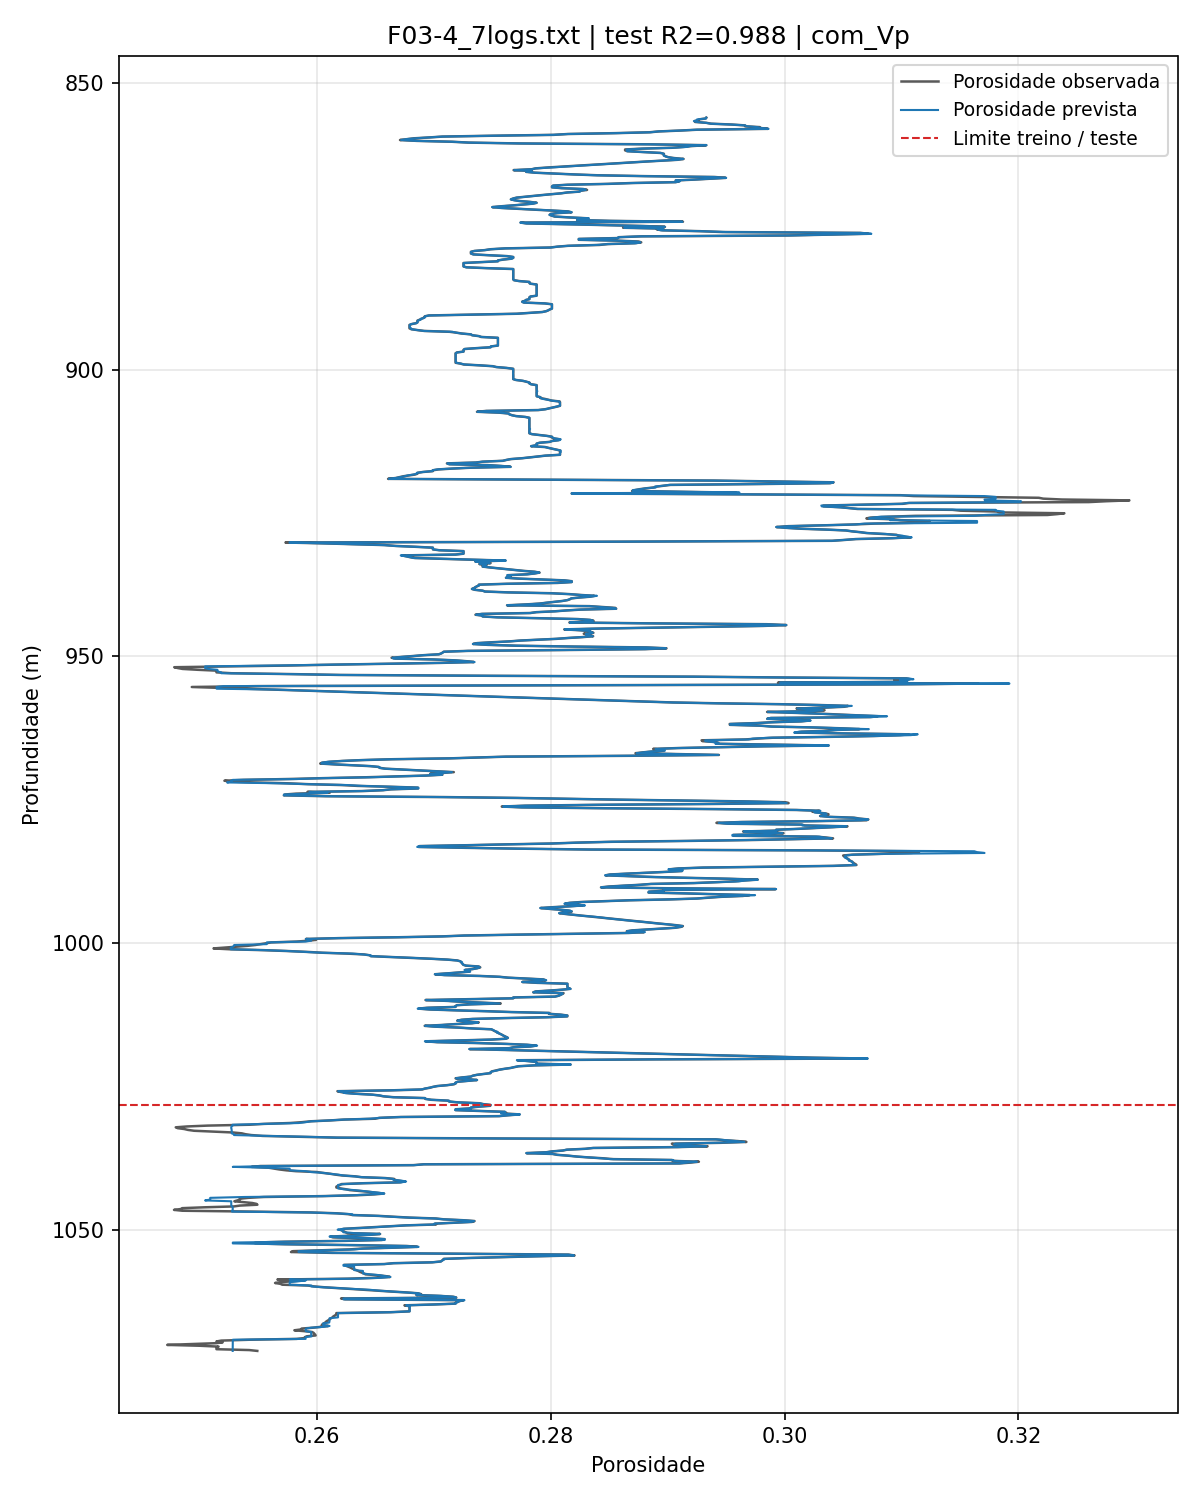
\includegraphics[width=0.85\textwidth]{porosity_F03-4_com_Vp.png}
\caption{Recorte principal: porosidade observada e prevista com todos os preditores
elásticos disponíveis.}
\label{fig:f03vp}
\end{figure}

\begin{figure}[p]
\centering
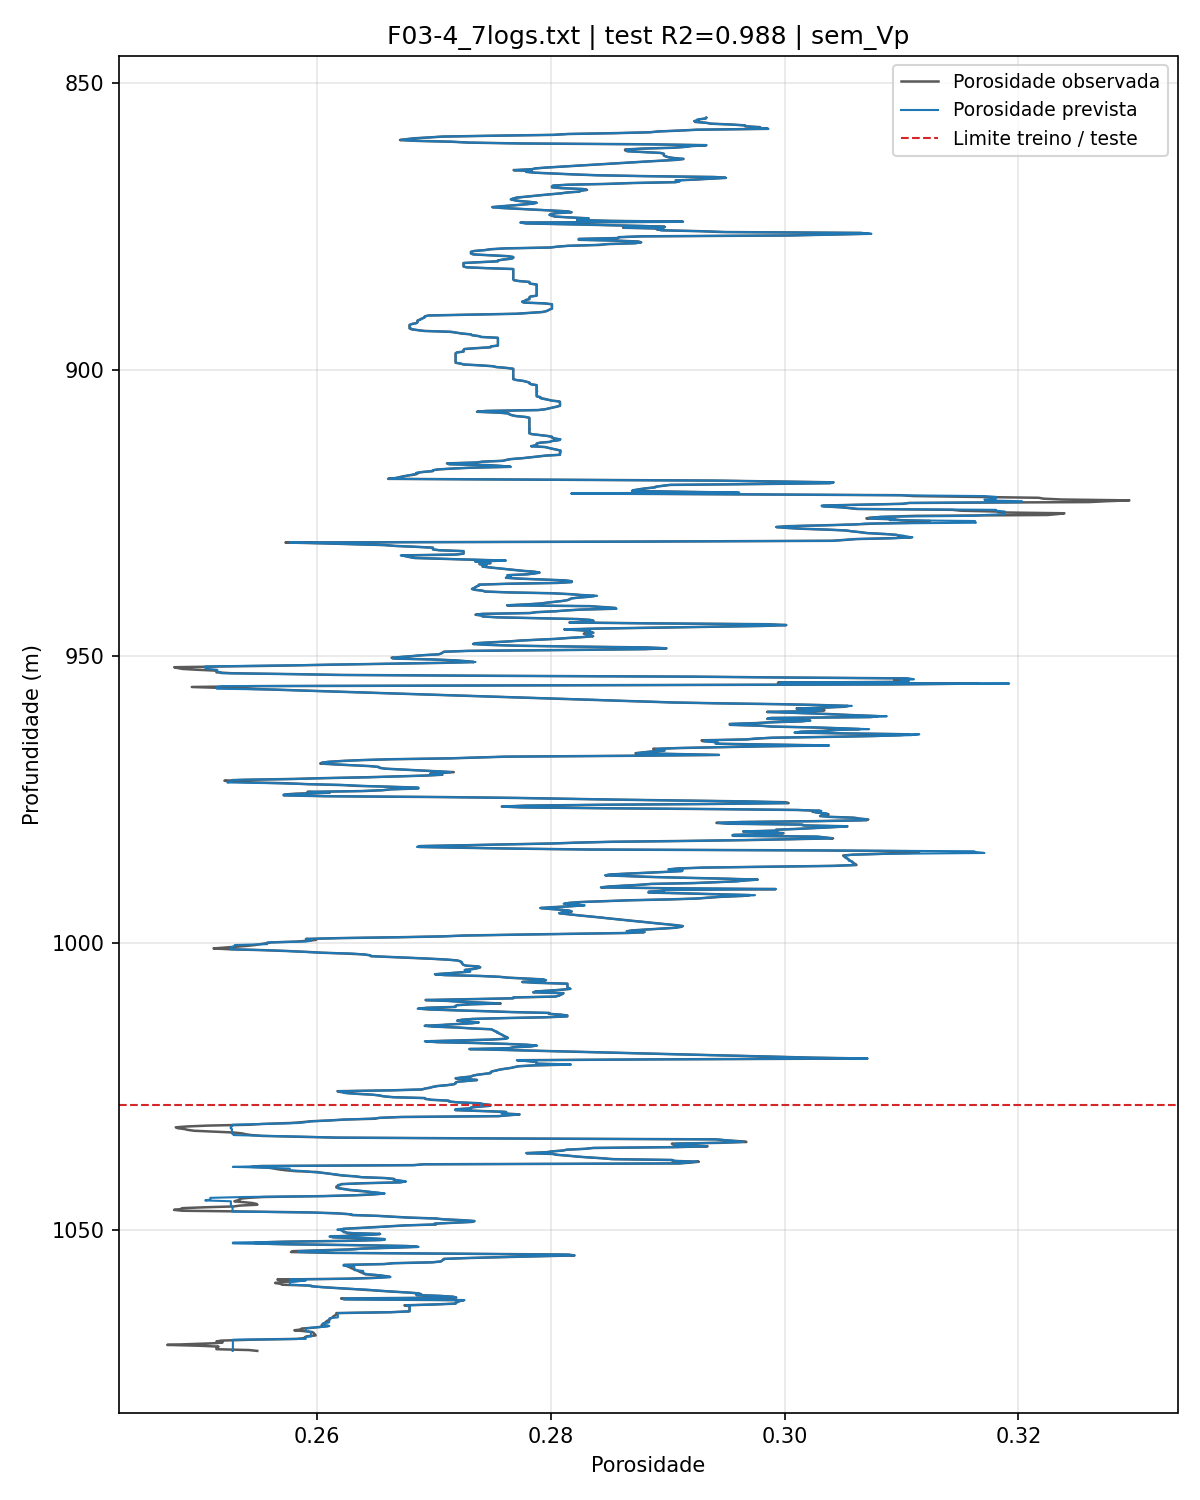
\includegraphics[width=0.85\textwidth]{porosity_F03-4_sem_Vp.png}
\caption{Recorte principal: modelo sem \(V_p\).}
\label{fig:f03svp}
\end{figure}

\begin{figure}[p]
\centering
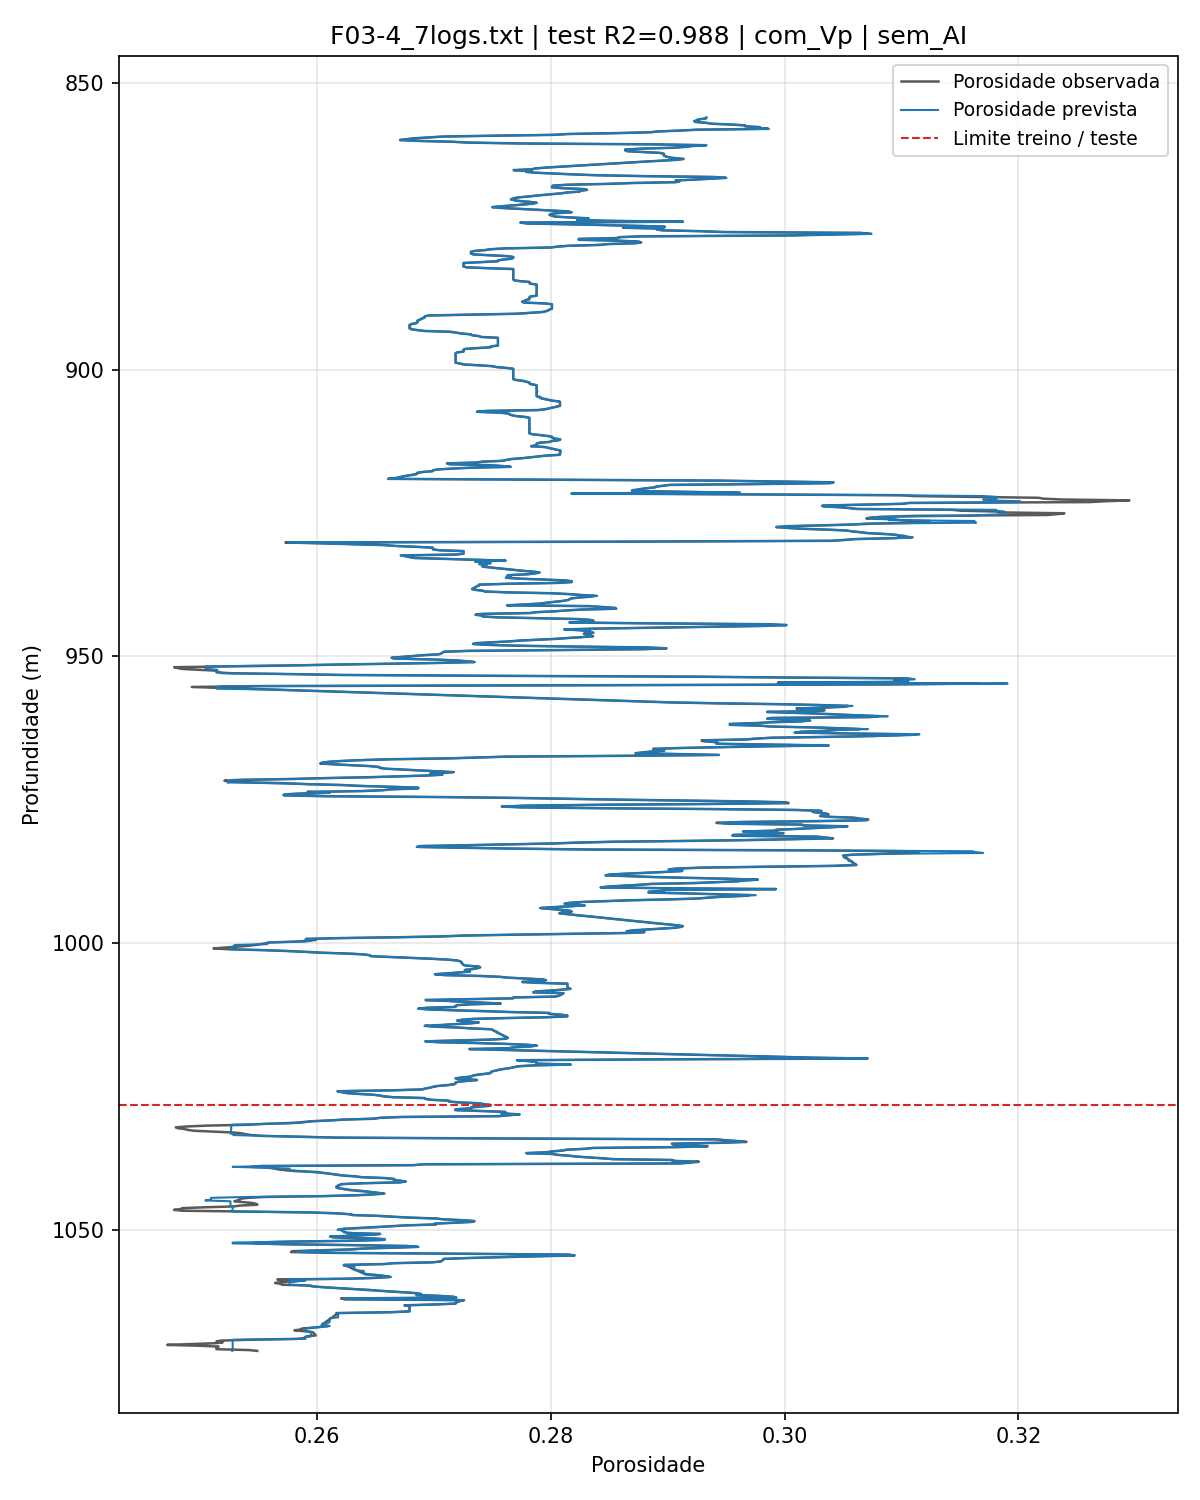
\includegraphics[width=0.85\textwidth]{porosity_F03-4_sem_AI.png}
\caption{Recorte principal: modelo sem impedância acústica.}
\label{fig:f03sai}
\end{figure}

\begin{figure}[p]
\centering
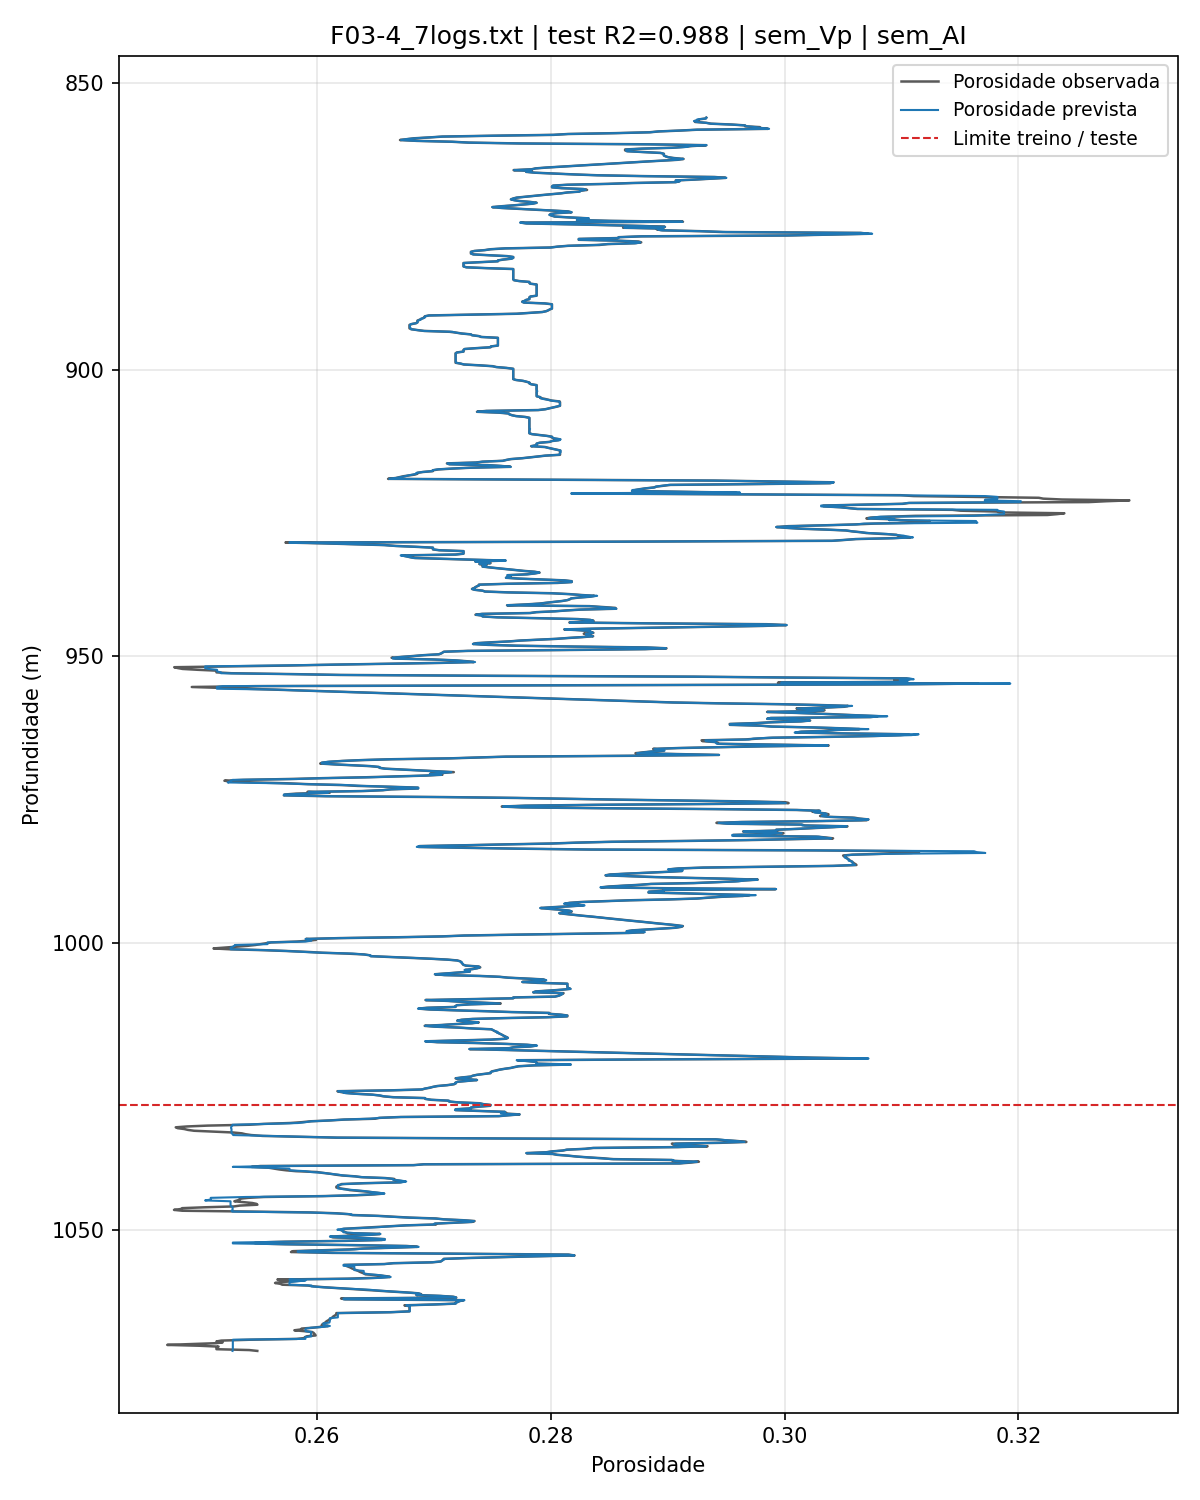
\includegraphics[width=0.85\textwidth]{porosity_F03-4_sem_Vp_sem_AI.png}
\caption{Recorte principal: modelo apenas com AC, \(\rho_b\), GR e \(V_c\).}
\label{fig:f03svpai}
\end{figure}

\begin{figure}[p]
\centering
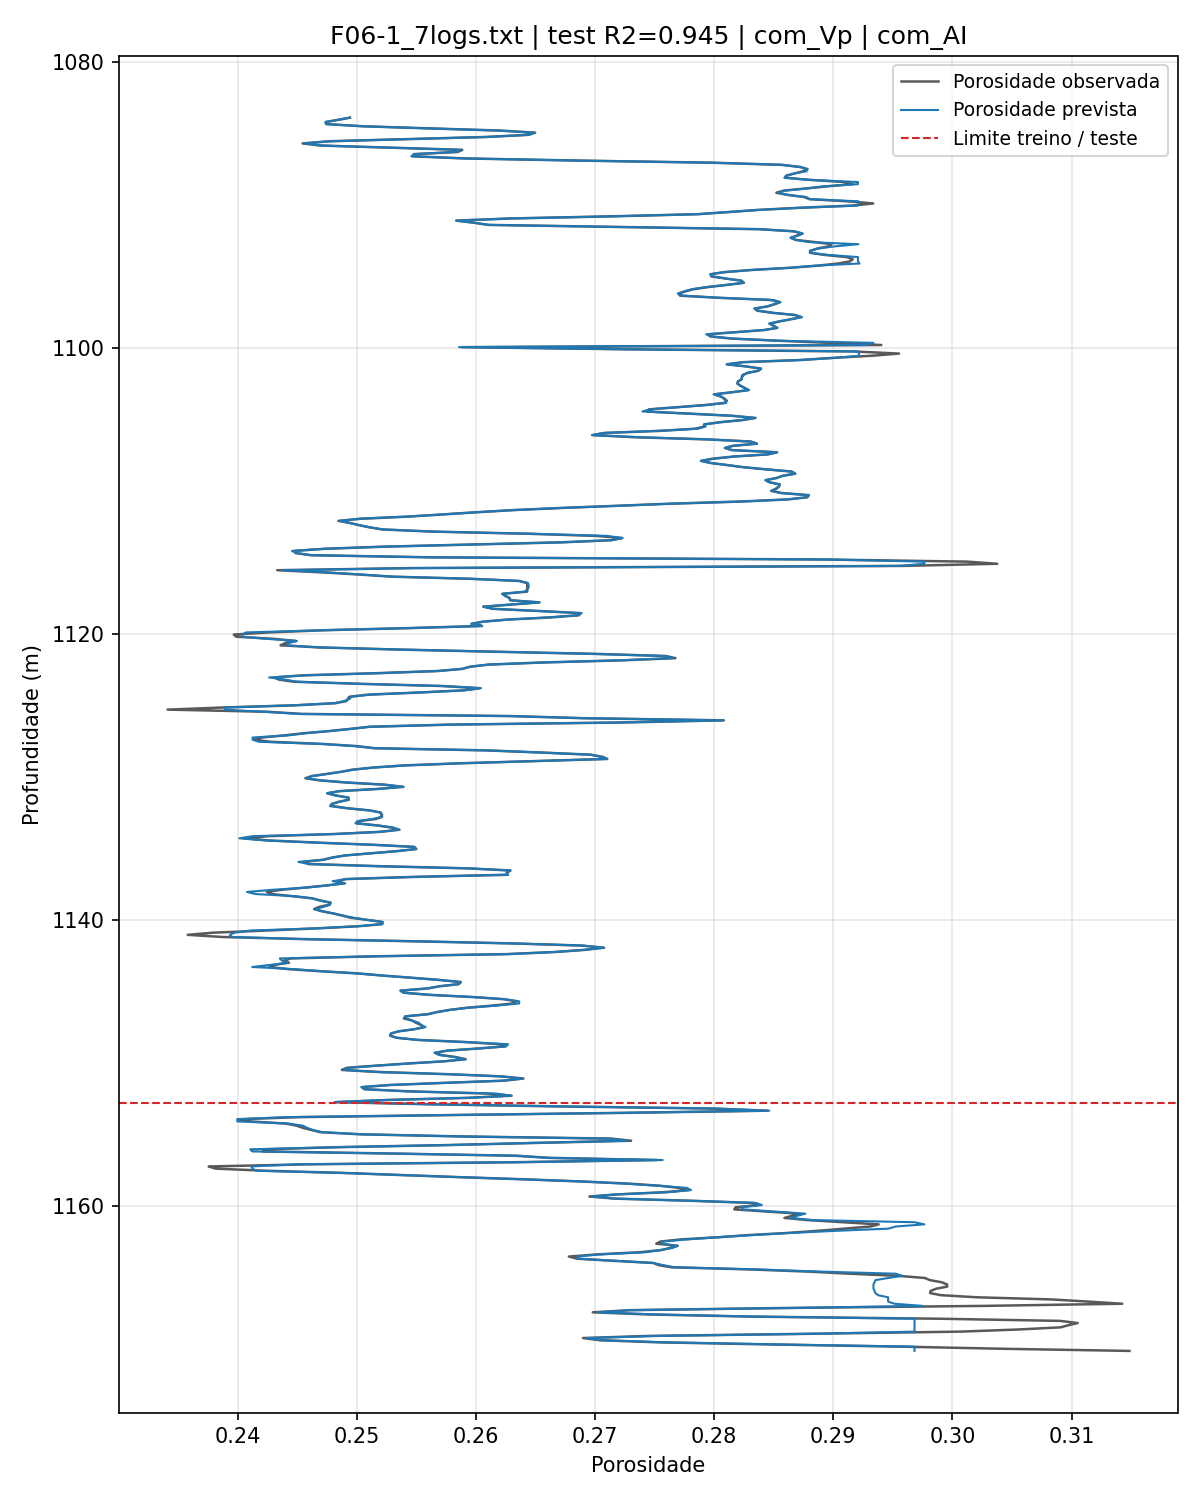
\includegraphics[width=0.85\textwidth]{porosity_F06-1_com_Vp.png}
\caption{Recorte de contraste: baseline completa.}
\label{fig:f06}
\end{figure}

\subsection{Estrutura de correlação e colinearidade}
As Figuras~\ref{fig:pearson} e~\ref{fig:spearman} evidenciam correlações lineares
e monótonas quase unitárias entre AC, \(\rho_b\), impedância e \(V_p\), bem
como correlação forte deste bloco com a porosidade \textbf{no recorte principal}.
O padrão sustenta a hipótese de um subespaço elástico de dimensão efetiva
baixa neste conjunto: várias colunas movem-se em conjunto, em vez de oferecer
direções independentes no espaço das variáveis.

A Tabela~\ref{tab:vif} traduz essa leitura em termos de~\eqref{eq:vif}: fatores da
ordem de \(10^5\) a \(10^6\) para AC, \(\rho_b\), impedância e \(V_p\) não devem
ser tomados como magnitudes calibradas de um modelo linear final. Dado o nível
extremo de colinearidade, os \textbf{valores absolutos} de VIF perdem interesse
quantitativo fino e devem ser lidos apenas como \textbf{marcadores de degenerescência
severa} do sistema linear auxiliar; comparações finas entre, por exemplo,
\(7{,}0\times 10^5\) e \(1{,}1\times 10^5\) não devem ser interpretadas como diferença
substancial de ``grau de colinearidade''. Para GR e \(V_c\), os VIF permanecem elevados
face ao limiar usual da ordem de dez, coerente com a forte associação mútua
observada nas matrizes.

\begin{table}[h]
\centering
\begin{tabular}{lr}
\toprule
Preditor & VIF (ordem de grandeza) \\
\midrule
AC & $7{,}0 \times 10^5$ \\
$\rho_b$ & $7{,}0 \times 10^5$ \\
Impedância & $1{,}1 \times 10^5$ \\
$V_p$ & $1{,}1 \times 10^5$ \\
GR & $8{,}3 \times 10^1$ \\
$V_c$ & $8{,}2 \times 10^1$ \\
\bottomrule
\end{tabular}
\caption{Fatores VIF aproximados no recorte principal (treino, bloco raso), calculados por~\eqref{eq:vif}.}
\label{tab:vif}
\end{table}

\subsection{Dependência entre GR e \(V_c\): postos e empates}\label{subsec:grvc}
O par GR--\(V_c\) aparece nas matrizes de correlação com associação forte,
mas a leitura sob \textbf{empates nos postos} (vários pontos com o mesmo valor,
logo o mesmo posto após \textit{ranking}) e sob \textbf{desempates} extremos
(\textit{min} e \textit{max} na rotina de postos adotada) informa se a dependência seria
artefato numérico ou se permanece quase determinística.

No recorte principal, sobre o mesmo conjunto 7logs já filtrado por linhas
completas, calcularam-se estatísticas de empates, correlações de Pearson,
Spearman e Kendall, correlações parciais via correlação entre resíduos
de regressões lineares ordinárias (controlo pela profundidade; controlo adicional
pelo bloco elástico em bruto; variantes em que preditores e profundidade entram
como postos médios), e uma estabilidade de Spearman sob \textit{jitter} uniforme
minúsculo repetido (80 sorteios, escala da ordem de \(10^{-8}\) face à amplitude
das curvas). As tabelas seguintes consolidam os indicadores dessa etapa para o recorte
principal.

\begin{table}[h]
\centering
\begin{tabular}{lrrrr}
\toprule
Coluna & \(n\) & valores distintos & fração em empates & multiplicidade máx. \\
\midrule
GR & 1435 & 1110 & 0{,}298 & 23 \\
\(V_c\) & 1435 & 1110 & 0{,}298 & 23 \\
\bottomrule
\end{tabular}
\caption{Empates nos valores brutos: GR e \(V_c\) compartilham a mesma cardinalidade
de valores distintos e a mesma fração de linhas em empates (recorte principal).}
\label{tab:grvc_ties}
\end{table}

\begin{table}[h]
\centering
\small
\begin{tabular}{p{2.6cm} p{4.9cm} c}
\toprule
Medida & Notação / controlo & Valor \\
\midrule
Pearson (bruto) & \(\rho_{GR,Vc}\) & 0{,}993 \\
Spearman & \(\rho_S\) & 1{,}000 \\
Kendall & \(\tau\) & 1{,}000 \\
Parcial (bruto) & resíduos OLS; controlo: profundidade & 0{,}993 \\
Parcial (postos) & resíduos OLS em postos médios; controlo: posto(prof.) & 1{,}000 \\
Parcial (bruto) & resíduos OLS; controlo: AC, \(\rho_b\), AI, \(V_p\) & 0{,}992 \\
Parcial (postos) & postos médios; controlo: prof.\ e elásticos (postos) & 1{,}000 \\
Spearman + \textit{jitter} & média de 80 sorteios & 0{,}999992 \\
& desvio-padrão & \(8{,}6\times 10^{-7}\) \\
\bottomrule
\end{tabular}
\caption{Associação GR--\(V_c\) e correlações parciais lineares (resíduos
OLS; controlo \textbf{linear} apenas, sem equivalência a independência condicional geral).
Com monotonia empírica quase perfeita entre GR e \(V_c\), os \(p\)-valores
dos testes de Spearman e de Kendall (hipótese de independência) ficam abaixo do
que a aritmética de ponto flutuante distingue de zero, aparecendo como \(0\) na
tabela.}
\label{tab:grvc_assoc}
\end{table}

\begin{table}[h]
\centering
\small
\begin{tabular}{lccc}
\toprule
posto(GR) $\backslash$ posto(\(V_c\)) & \textit{average} & \textit{min} & \textit{max} \\
\midrule
\textit{average} & 1{,}000000 & 0{,}999991 & 0{,}999991 \\
\textit{min} & 0{,}999991 & 1{,}000000 & 0{,}999965 \\
\textit{max} & 0{,}999991 & 0{,}999965 & 1{,}000000 \\
\bottomrule
\end{tabular}
\caption{Sensibilidade ao desempate: Pearson entre postos obtidos com os métodos
\textit{average}, \textit{min} e \textit{max} de desempate; valores fora da diagonal diferem
só na sexta casa decimal.}
\label{tab:grvc_rankmethods}
\end{table}

A Tabela~\ref{tab:grvc_ties} mostra que GR e \(V_c\) não são meramente
correlacionados: compartilham \textbf{exatamente} o mesmo número de valores distintos,
a mesma fração de linhas em empates e a mesma multiplicidade máxima, o que
é compatível com \(V_c\) construído a partir de GR (ou inversamente) com a
mesma grelha de quantização. A Tabela~\ref{tab:grvc_assoc} confirma uma relação
quase monótona perfeita (Spearman e Kendall unitários) e mantém correlação
parcial elevada mesmo depois de linearizar profundidade ou o bloco elástico, pelo
menos no esquema de controlo linear adotado. Uma regressão isotônica crescente
\(V_c \approx f(\mathrm{GR})\) ajustada aos mesmos dados atinge \(R^2\) praticamente
unitário e erro de reconstrução desprezível à escala da precisão finita do cálculo, o que
quantifica a redundância monótona além das correlações clássicas. \textbf{No recorte principal, GR e \(V_c\)
não devem ser tratados como eixos independentes de informação:} a evidência
sugere que um deles é, na prática, quase inteiramente reconstruível a partir do
outro, de modo que mantê-los simultaneamente pode inflar artificialmente a dimensão
aparente do espaço de atributos. A Tabela~\ref{tab:grvc_rankmethods} mostra que a
escolha de desempate (\textit{average}, \textit{min}, \textit{max}) quase não move o
coeficiente; o \textit{jitter} deixa a Spearman estável na unidade até \(10^{-6}\).

\begin{figure}[p]
\centering
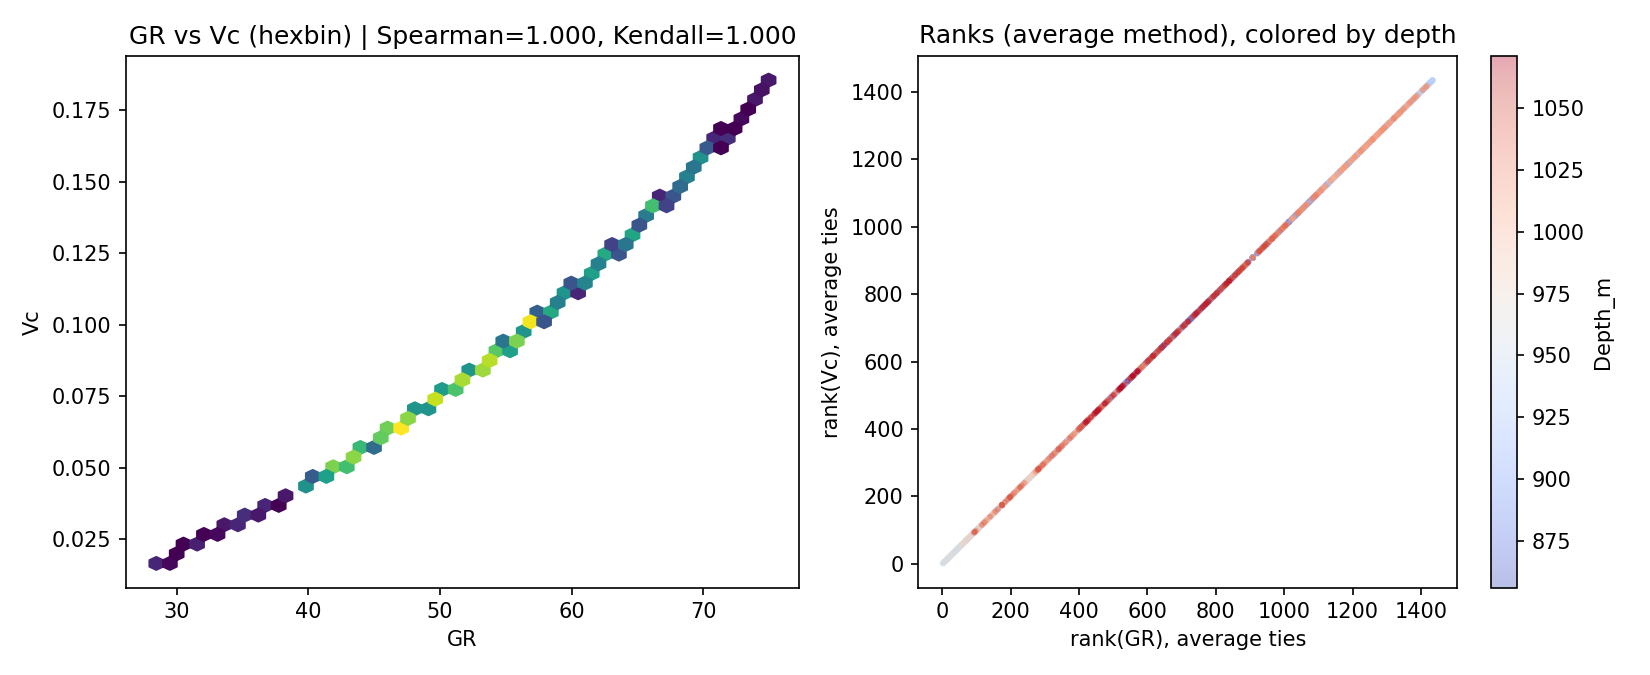
\includegraphics[width=\textwidth]{gr_vc_F03-4_ranks_scatter.png}
\caption{GR versus \(V_c\) (hexbin) e postos médios com cores por profundidade.
Spearman e Kendall próximos de um indicam monotonia quase perfeita no recorte.}
\label{fig:grvc_scatter}
\end{figure}

\begin{figure}[p]
\centering
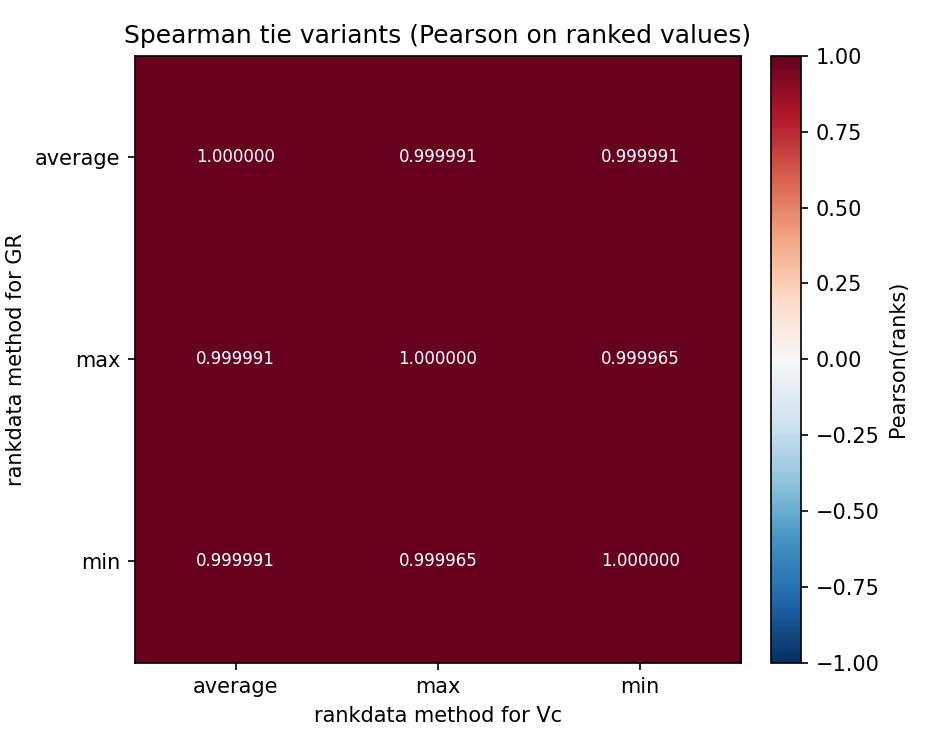
\includegraphics[width=0.62\textwidth]{gr_vc_F03-4_rank_method_sensitivity.png}
\caption{Mapa de calor da matriz da Tabela~\ref{tab:grvc_rankmethods}: sensibilidade
da correlação de Pearson aplicada a pares de postos, com coeficientes anotados
em cada célula (seis casas decimais).}
\label{fig:grvc_methods}
\end{figure}

\subsection{Informação mútua, permutação e SHAP}
A informação mútua (MI) entre cada preditor e a porosidade concentra-se em valores
elevados e muito próximos entre si para AC, \(\rho_b\), impedância e \(V_p\),
enquanto GR e \(V_c\) ficam num patamar inferior, porém não nulos. A leitura
relevante da MI é \textbf{ordinal e comparativa} entre preditores (ordenação e
separação entre blocos), e não o valor absoluto em nats como grandeza
transportável entre estudos. A Tabela~\ref{tab:mi_por} quantifica essa separação:
os quatro preditores elásticos
ficam na casa de \(5{,}3\) nats (arredondamento à segunda casa; MI estimada no treino), enquanto GR e
\(V_c\) permanecem perto de \(0{,}51\), isto é, magnitudes cerca de dez vezes
menores no mesmo ajuste MI. Isto reforça que, \textbf{no recorte principal}, o
bloco elástico compartilha quase o mesmo conteúdo informativo sobre o alvo, ao
passo que GR e \(V_c\) introduzem um eixo litológico mais fraco neste recorte, sem
ser nulo.

\begin{table}[h]
\centering
\begin{tabular}{lr}
\toprule
Preditor & MI com porosidade (nats, arred.) \\
\midrule
AC & 5{,}30 \\
\(\rho_b\) & 5{,}43 \\
AI & 5{,}28 \\
\(V_p\) & 5{,}30 \\
GR & 0{,}52 \\
\(V_c\) & 0{,}51 \\
\bottomrule
\end{tabular}
\caption{MI estimada no conjunto de treino (bloco raso, mesma partição que as
Figuras~\ref{fig:pearson}--\ref{fig:spearman}). Valores arredondados; ver limitações na
Secção~\ref{sec:premissas}.}
\label{tab:mi_por}
\end{table}

A Figura~\ref{fig:perm} sintetiza a importância por permutação (25 repetições
no teste profundo). A Tabela~\ref{tab:perm_r2} traduz a figura em números: a queda
média de \(R^2\) ao baralhar AC é da ordem de \(1{,}30\), com desvio-padrão de
\(0{,}06\), enquanto \(\rho_b\) aparece distante, mas ainda positiva (\(\approx 0{,}05\)).
AI e \(V_p\) têm quedas médias uma ordem de grandeza menores; \(V_p\) fica na casa
de \(10^{-5}\), compatível com ausência de contribuição marginal detectável
à escala do ruído de permutação. GR exibe média ligeiramente negativa
(\(\approx -9\times 10^{-4}\)), compatível com flutuação estatística em torno
de zero quando o preditor é redundante; \(V_c\) registra queda média nula à
resolução numérica utilizada na tabela, coerente com o acoplamento quase determinístico a GR já
documentado.

Em presença de colinearidade forte, a importância por permutação mede
contribuição \textbf{marginal} condicionada ao restante dos preditores e, por
construção, tende a \textbf{subestimar} variáveis cuja informação já foi
absorvida por colunas correlacionadas; quedas quase nulas em AI e \(V_p\) não
equivalem a ausência física de conteúdo informativo, mas sim a redundância
preditiva face a AC e \(\rho_b\) neste ajuste.

\begin{table}[h]
\centering
\small
\begin{tabular}{lcc}
\toprule
Preditor & Queda média de \(R^2\) & Desvio-padrão \\
\midrule
AC & 1{,}298 & 0{,}064 \\
\(\rho_b\) & 0{,}050 & 0{,}005 \\
AI & 0{,}0056 & 0{,}0010 \\
\(V_p\) & \(2{,}9\times 10^{-5}\) & \(3{,}4\times 10^{-6}\) \\
GR & \(-9{,}1\times 10^{-4}\) & \(3{,}3\times 10^{-4}\) \\
\(V_c\) & 0{,}000 & 0{,}000 \\
\bottomrule
\end{tabular}
\caption{Importância por permutação no teste profundo (25 repetições). Registou-se,
em paralelo à tabela, um indicador binário que assinala preditores cuja queda média de
\(R^2\) não é positiva, para facilitar a leitura de redundância ou ruído à escala do procedimento.}
\label{tab:perm_r2}
\end{table}

A Figura~\ref{fig:shap}, no mesmo modelo GBDT e no recorte principal, mostra que AC
emerge como o principal \textbf{carregador de informação preditiva marginal} na
base explicada: a nuvem de SHAP para AC ocupa faixa horizontal visivelmente mais larga
do que as de AI, \(V_p\) e \(\rho_b\), sinal de que pequenas variações de AC se
traduzem em variações grandes no valor de Shapley ao longo das observações
do teste. Isto não atribui a AC o papel de ``variável certa'' em sentido absoluto,
apenas descreve o modelo ajustado neste protocolo. AI e
\(V_p\) aparecem como faixas estreitas centradas perto de zero, coerente com a
redundância frente a AC e densidade. \(\rho_b\) mostra dispersão intermediária,
refletindo o papel secundário mas não nulo visto na permutação. GR e \(V_c\)
mantém dispersão modesta e parcialmente sobreposta, alinhada à MI baixa e à
quase colinearidade entre si: o SHAP deve ser lido como explicação \textit{local}
do ajuste, não como atribuição causal física.

\begin{figure}[p]
\centering
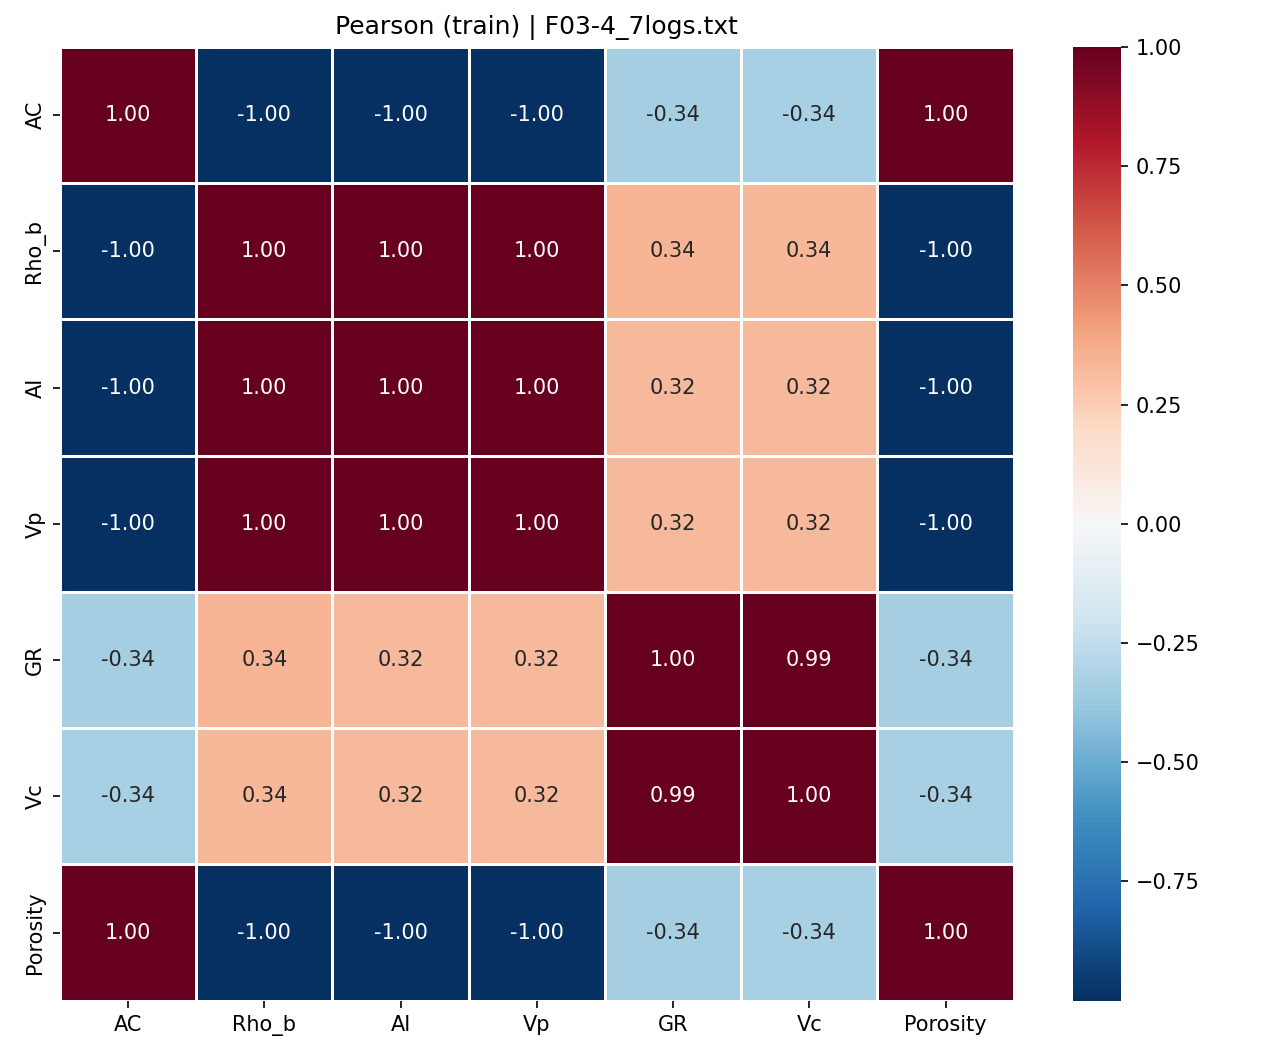
\includegraphics[width=\textwidth]{study_F03-4_corr_pearson.png}
\caption{Correlações de Pearson entre preditores e porosidade (recorte principal).}
\label{fig:pearson}
\end{figure}

\begin{figure}[p]
\centering
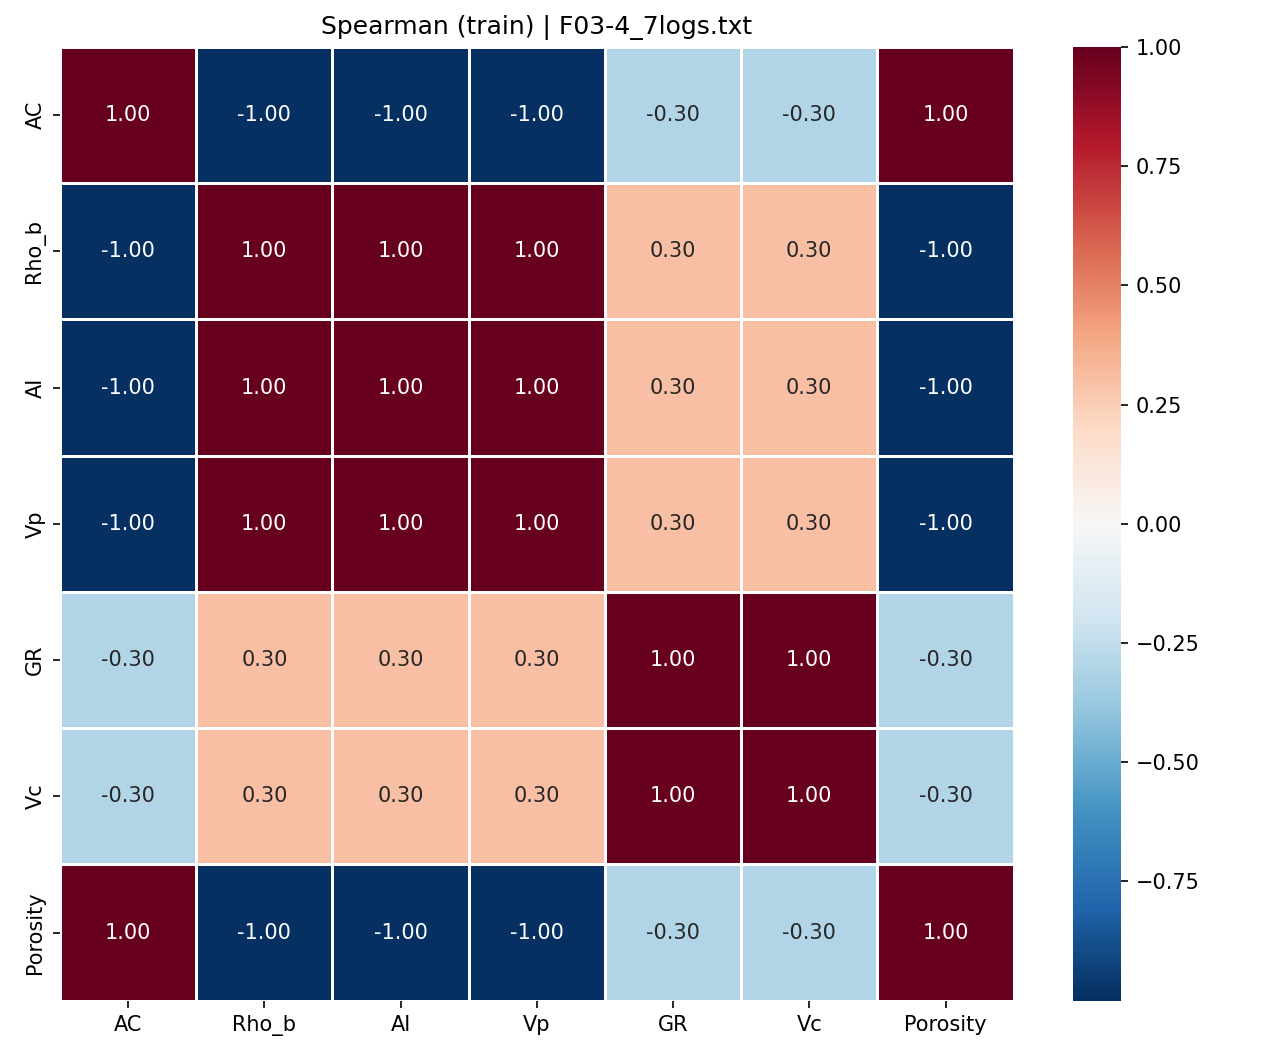
\includegraphics[width=\textwidth]{study_F03-4_corr_spearman.png}
\caption{Correlações de Spearman (recorte principal).}
\label{fig:spearman}
\end{figure}

\begin{figure}[p]
\centering
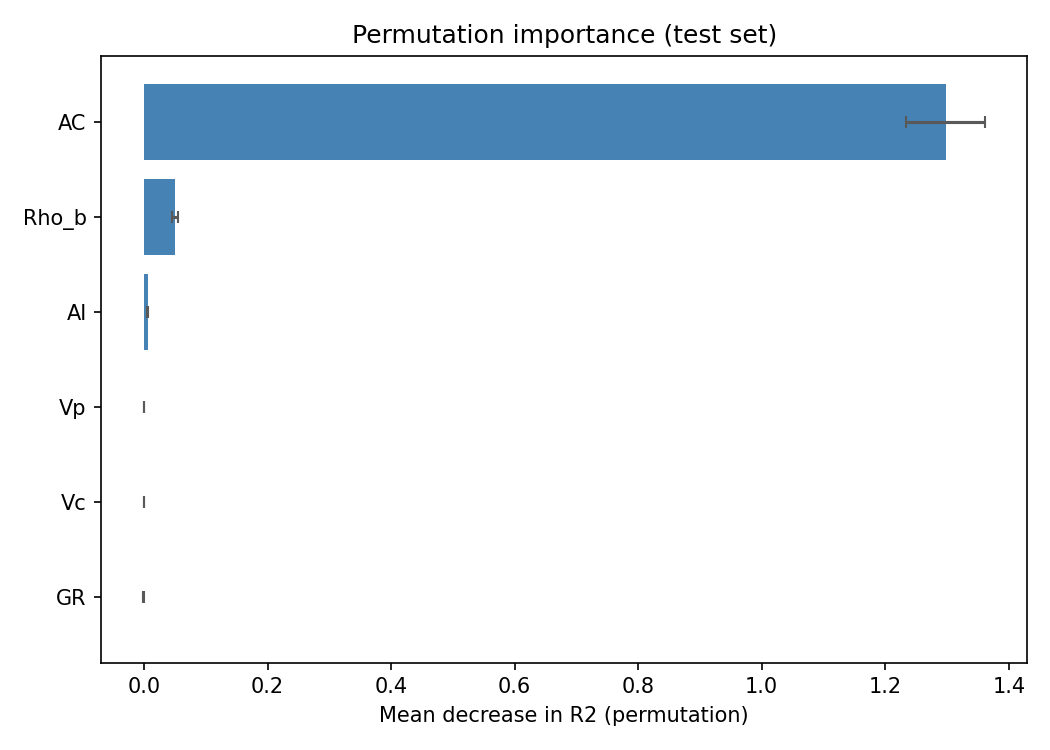
\includegraphics[width=0.92\textwidth]{study_F03-4_perm_importance.png}
\caption{Importância por permutação: queda média de \(R^2\) no teste ao
baralhar cada preditor.}
\label{fig:perm}
\end{figure}

\begin{figure}[p]
\centering
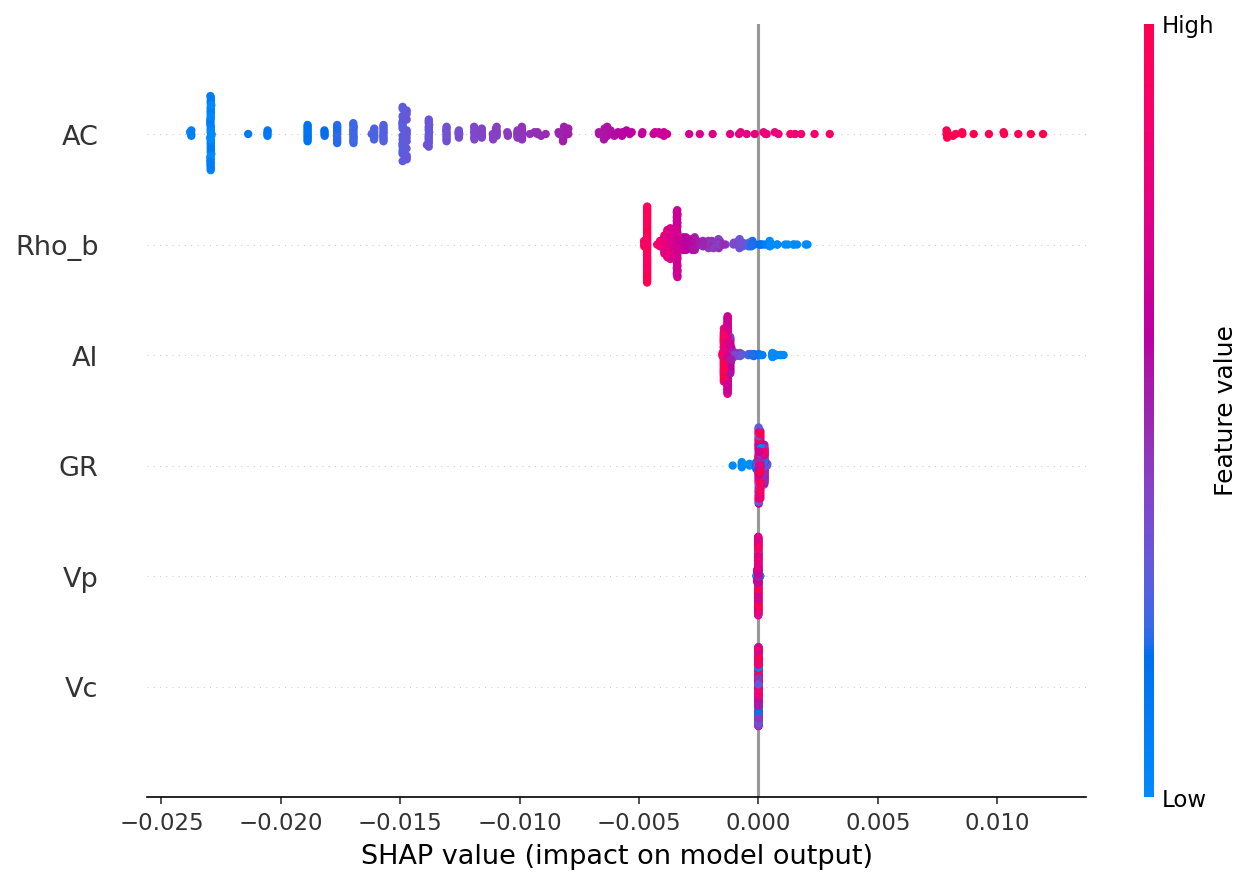
\includegraphics[width=\textwidth]{study_F03-4_shap_summary.png}
\caption{Resumo SHAP (\textit{SHapley Additive exPlanations}) no conjunto de teste
profundo (287 observações).}
\label{fig:shap}
\end{figure}

\section{Discussão}\label{sec:discussao}

A estabilidade das métricas na Tabela~\ref{tab:metricas}, percorrida em paralelo
com as ablações ilustradas nas Figuras~\ref{fig:f03svp}--\ref{fig:f03svpai},
indica que, \textbf{no recorte principal} e sob o protocolo treino/teste em profundidade,
\(V_p\) e a impedância não acrescentam \textbf{ganho preditivo marginal detectável}
quando AC e \(\rho_b\) já estão disponíveis com a qualidade relativa destas
curvas. Não se trata de desvalorizar medidas físicas centrais: o experimento não
implica irrelevância física de \(V_p\) ou de AI, mas sim ausência de contribuição
preditiva marginal detectável neste contexto, dado o forte acoplamento dessas
grandezas com AC e densidade.

A Secção~\ref{sec:resultados} fornece a evidência multivariada que sustenta
esta leitura: correlações quase unitárias no bloco elástico
(Figuras~\ref{fig:pearson} e~\ref{fig:spearman}), VIF extremos na
Tabela~\ref{tab:vif}, MI ordenada como na Tabela~\ref{tab:mi_por}, quedas de \(R^2\)
por permutação como na Tabela~\ref{tab:perm_r2} e na Figura~\ref{fig:perm}, e
resumo SHAP (Figura~\ref{fig:shap}) coerente com essa hierarquia. Em conjunto, estas
linhas de evidência fecham o ciclo lógico entre a pergunta formulada na
Secção~\ref{sec:perguntas} e o desenho metodológico da Figura~\ref{fig:fluxo}.

A subsecção~\ref{subsec:grvc} aprofunda o par GR--\(V_c\) sob a ótica de empates
nos postos e de desempates extremos. As Tabelas~\ref{tab:grvc_ties}--\ref{tab:grvc_rankmethods}
e as Figuras~\ref{fig:grvc_scatter} e~\ref{fig:grvc_methods} mostram estrutura de
empates idêntica entre colunas, Spearman e Kendall próximos de um e correlação
parcial ainda elevada após controlo linear pela profundidade ou pelo bloco elástico,
o que reforça que, neste recorte, GR e \(V_c\) não funcionam como preditores
litológicos independentes no espaço de entrada.

O contraste com a Figura~\ref{fig:f06} e a última linha da Tabela~\ref{tab:metricas}
mostra que o nível de \(R^2\) não é propriedade universal do modelo: depende
do recorte. Daí a cautela ao extrapolar conclusões entre colunas distintas sem
protocolo de exclusão mútua no treino.

\paragraph{Contraste entre recortes F03-4 e F06-1.}
No recorte principal (F03-4), após remoção de linhas incompletas, restam
\(n=1435\) profundidades entre \(856\) e \(1071\,\mathrm{m}\), com porosidade média
\(0{,}278\) e desvio-padrão \(0{,}014\). No recorte de contraste (F06-1), \(n=576\)
entre \(1084\) e \(1170\,\mathrm{m}\), com porosidade média \(0{,}267\) e desvio
\(0{,}017\). A janela vertical é distinta e o segundo conjunto é menor; a
porosidade apresenta dispersão relativa ligeiramente maior no F06-1. Estes fatos
não explicam por si sós toda a queda de \(R^2\) na Tabela~\ref{tab:metricas}, mas
mostram que o teste profundo (20\%) corresponde a litologias, profundidades e
tamanhos amostrais diferentes, pelo que o \(R^2\) deixa de ser comparável como se
fosse repetição do mesmo experimento. Complementou-se essa comparação com o
bootstrap pareado da Secção~\ref{subsec:bootstrap_test} (Tabela~\ref{tab:bootstrap_ic}):
os intervalos aproximados a \(95\%\) para \(R^2\) \textbf{não se sobrepêm} entre
F03-4 e F06-1 (limite superior \(0{,}9679\) versus limite inferior \(0{,}9829\)), o que
sustenta que a diferença pontual entre \(0{,}988\) e \(0{,}945\) não se explica
apenas por flutuação de amostragem \textit{dentro} de cada coluna sob esta
reamostragem. O aviso metodológico permanece: estes intervalos não substituem
validação por exclusão de poço.

\paragraph{Limite principal.}
O ensaio caracteriza \textbf{robustez interna} ao recorte e ao protocolo adotado; não
caracteriza \textbf{transferência entre poços} nem domínio geológico alargado.
O teste profundo, por mais exigente que seja face a um sorteio i.i.d., permanece
intra-coluna: esta limitação deve pesar em qualquer extrapolação além do
material tabular analisado.

\section{Conclusões}\label{sec:conclusoes}

No recorte principal, o modelo atinge \(R^2\) elevado no teste profundo e mantém
esse desempenho ao remover \(V_p\) ou impedância, o que é explicado, não
contradito, pela colinearidade forte documentada nas Figuras~\ref{fig:pearson}
e~\ref{fig:spearman} e pelos VIF da Tabela~\ref{tab:vif}. A MI (Tabela~\ref{tab:mi_por})
e as quedas de \(R^2\) por permutação (Tabela~\ref{tab:perm_r2} e
Figura~\ref{fig:perm}), juntamente com o SHAP (Figura~\ref{fig:shap}), indicam que,
\textbf{no modelo ajustado e neste recorte}, AC emerge como o principal carregador de
informação preditiva marginal, enquanto a maior parte da variância explicada no
teste flui por um eixo elástico estreito no qual AI e \(V_p\) ficam preditivamente
redundantes face a AC e \(\rho_b\), sem afastar a sua relevância física em outros
contextos ou com outras qualidades de aquisição.

O recorte de contraste lembra que a generalização espacial ou entre contextos
exige desenho experimental próprio; o presente ensaio não o substitui. Os IC de
bootstrap no teste (Tabela~\ref{tab:bootstrap_ic}) reforçam que o contraste de
\(R^2\) entre recortes não é compatível com intervalos sobrepostos sob a
reamostragem adotada, sem por isso afastar a necessidade de protocolos entre poços.
A revisão de dependência entre GR e \(V_c\) sob postos e empates
(Secção~\ref{subsec:grvc}) confirma quase redundância formal entre esses
preditores no recorte principal.

O ensaio caracteriza robustez interna ao recorte e \textbf{não} transferência entre
poços; esta última permanece etapa futura necessária. Como próximos passos,
\textbf{recomenda-se}: (i) validação LOO (\textit{leave-one-well-out}) ou equivalente com
exclusão mútua de poços no treino; (ii) repetição do mesmo protocolo em
múltiplos recortes e múltiplas colunas, para verificar estabilidade do diagnóstico
de redundância; (iii) quando possível, substituir ou complementar a porosidade-alvo
por referência menos acoplada às curvas elásticas usadas como entrada.

\section*{Referências}

\begin{itemize}
  \item Pedregosa et al., Scikit-learn: Machine Learning in Python, \textit{Journal of Machine Learning Research}, 2011.
  \item Lundberg, S. M.; Lee, S.-I., A Unified Approach to Interpreting Model Predictions,
  \textit{Conference on Neural Information Processing Systems} (NeurIPS), 2017.
\end{itemize}

\end{document}
